\documentclass{article}
\usepackage{graphicx,amsmath}
\usepackage{fullpage}


\let\a=\alpha \let\b=\beta  \let\g=\gamma  \let\d=\delta \let\e=\varepsilon
\let\z=\zeta  \let\h=\eta   \let\th=\theta \let\k=\kappa \let\l=\lambda
\let\m=\mu    \let\n=\nu    \let\x=\xi     \let\p=\pi    \let\r=\rho
\let\s=\sigma \let\t=\tau   \let\f=\varphi \let\ph=\varphi\let\c=\chi
\let\ps=\psi  \let\y=\upsilon \let\o=\omega\let\si=\varsigma
\let\G=\Gamma \let\D=\Delta  \let\Th=\Theta\let\L=\Lambda \let\X=\Xi
\let\P=\Pi    \let\Si=\Sigma \let\F=\Phi    \let\Ps=\Psi
\let\O=\Omega \let\Y=\Upsilon
\let\ee=\epsilon

\def\DD{{\cal D}}
\newcommand{\beq}{\begin{equation}}
\newcommand{\eeq}{\end{equation}}
\def\de{\mathrm d}
\let\io=\infty 
\def\la{\left\langle}
\def\ra{\right\rangle}



\begin{document}
\begin{flushleft}
{\bf \Large From Statistical Physics  to Data-Driven Modelling \\ with Applications in Quantitative Biology : Tutorial 1} 
\hskip 0.1 cm S.C., R.M., F.Z. 
\vskip .3cm
{\bf \Large  Bayesian inference and single-particle tracking}
\vskip .3cm
{\bf \Large  Corrections}
\vskip .3cm
\hrule
\vskip .3cm
\end{flushleft}

\noindent

\subsection*{Solution}

\subsubsection*{Data Analysis}

The trajectory in the $(x,y)$ plane given in the data for $M=1000$ is plotted in figure~\ref{trag} (left). It has the characteristics of a random-walk: the space is not regularly filled, 
but  the trajectory densely explore one region before ``jumping'' to another region.

\begin{figure}[h]
\centering
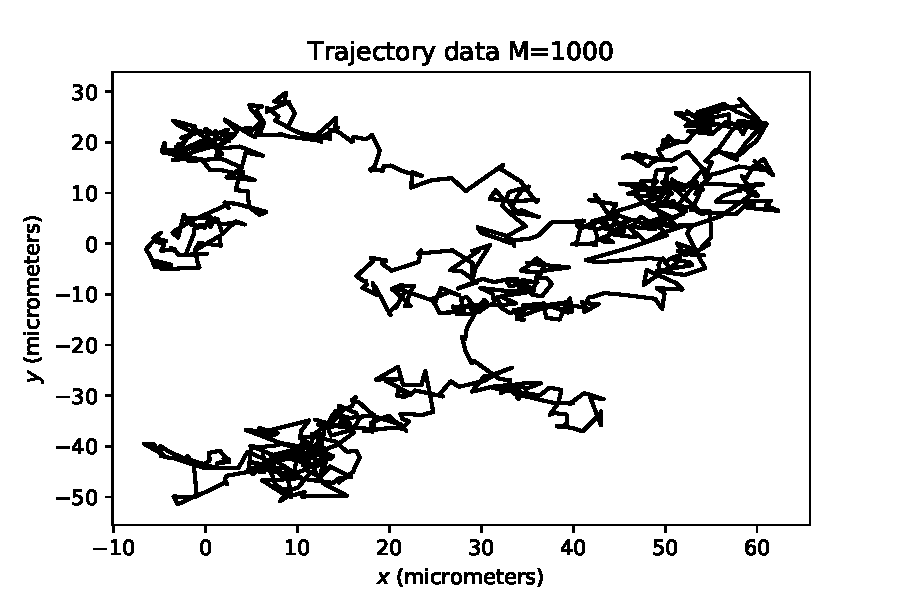
\includegraphics[width=.49\textwidth]{Figs1/trajectory_dataM1000d2_5.pdf}
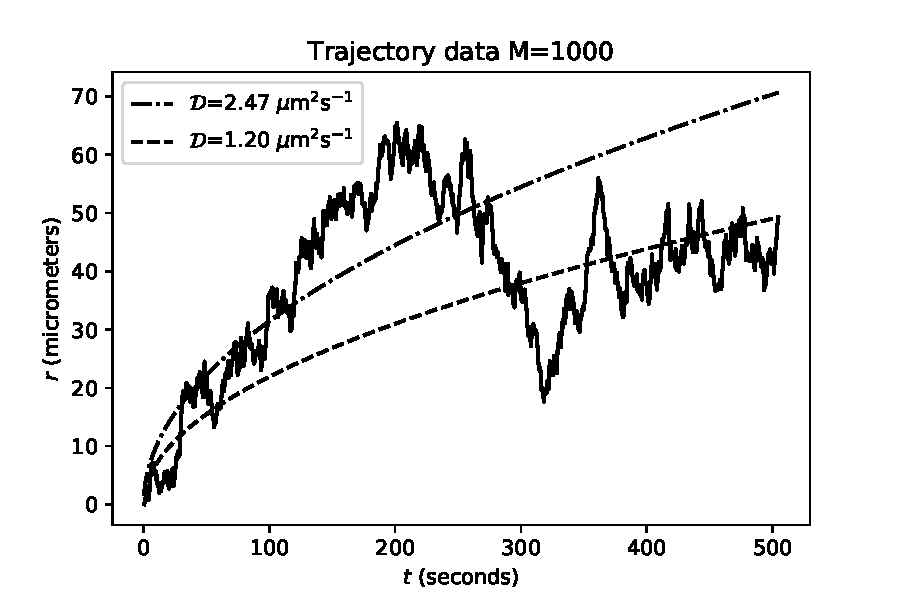
\includegraphics[width=.49\textwidth]{Figs1/rvst_dataM1000d2_5.pdf}
\caption{Left: trajectory of the particle. Right: displacement  from the origin as a function of time.}
\label{trag}
\end{figure}
 
 The displacement $r=\sqrt {x^2+y^2}$ as a function of time is plotted in figure~\ref{trag} (right). On average, it grows as the square root of the time, but on a single trajectory we observe large fluctuations. 
 The random walk in two dimensions is described by the relation:
\begin{equation}
\langle r^2(t) \rangle= 4 \DD t \ ,
 \end{equation}
where $\DD$ is the diffusion coefficient whose physical dimensions are  ${[\DD]=l^2 t^{-1}}$. Here lengths are given in $\mu$m and times in s.
A first estimate of $\DD$ from the data can be obtained by just considering the largest time and estimating
\begin{equation}
\DD_0 = \frac{r^2(t_{max})}{4 t_{max}}
\end{equation}
giving $\DD_0=1.20 \mu m^2\;s^{-1}$ for the data set with $M=1000$.
Another estimate of $\DD$ can be obtained as the average of the square displacement from one data point to the next one divided by the time interval.
 We define the differences between two successive positions and between two successive recording times
  \beq
 \delta x_i=x_{i+1}-x_i \ ,\qquad \delta y_i=y_{i+1}-y_i \ , \qquad \delta t_i=t_{i+1}-t_i \ .
 \eeq 
 Note that $i=1,\ldots, M-1$. The  square displacement in a time step is  $\delta r_i^2= \delta x_i^2+\delta y_i^2 $ and the estimate of $\DD$ is
 \begin{equation}
 \DD_1=\frac {1}{4 (M-1)}\sum_{i=1}^{M-1} \frac{ \delta r_i^2}{\delta t_i} \ ,
 \end{equation}
 giving $\DD_1=2.47 \mu m^2\;s^{-1}$ for the same data set.
 These estimates are compared with the trajectory in figure~\ref{trag} (right).



\subsubsection*{Posterior distribution}

%We consider a particle undergoing diffusive motion in the plane, with position $\vec r(t) = \big(  \tilde x(t),  \tilde y(t)\big)$ at time $t$. The diffusion coefficient (supposed to be isotropic) is denoted by $\DD$, and we assume that the average velocity vanishes. Measurements give access to the positions $x_i,y_i$ of the particles at times $t_i$, where $i$ is a positive integer running from 1 to $N$,

 Due to diffusion $\delta x_i$ and $\delta y_i$ are Gaussian random variables with variances $2\DD \,\delta t_i$.   We have
\begin{equation}
p(\delta x_i|\DD,\d t_i)=\frac{1}{\sqrt {4\pi \DD\,\delta t_i} } e^ {-\frac{\delta x_i^2 }{ 4\,\DD\,\delta t_i}} \ ,
\end{equation}
and  $p(\delta y_i | \DD,\d t_i)$ has the same form.
 The probability of a time series of increments ${\{ \d x_i, \d y_i\}_{i=1,...,M-1}}$, given $\DD$ is therefore:
 \begin{equation}\begin{split}
P(\{ \d x_i, \d y_i\}|\DD, \{\d t_i \}) &= \prod_{i=1}^{M-1}\frac{1}{ {4\pi \DD\,\delta t_i} } e^ {-\frac{\delta x_i^2 }{ 4\,\DD\,\delta t_i}- \frac{\delta y_i^2 }{ 4\,\DD\,\delta t_i}} \\
&= C e^{-B/\DD} \, \DD^{-(M-1)} \ ,
\end{split}\end{equation}
where $C={\prod_{i=1}^{M-1}\frac 1 {4\pi\delta t_i} }$ and $B=\sum_{i=1}^{M-1} \frac{\delta r_i^2  }{ 4\,\delta t_i}$.
Note that to infer $\DD$ we do not need the absolute values of $(x_i, y_i)$, but only their increments on each time interval.

According to Bayes'  Theorem,
\begin{equation}
P(\DD|\{ \d x_i, \d y_i, \d t_i\})= \frac{P(\{ \d x_i, \d y_i\}|\DD,\{\d t_i\}) P(\DD)}{\int_0^{\infty}  \de \DD \;P(\{ x_i,y_i\}|\DD,\{\d t_i \}) P(\DD)} \ .
\end{equation}
We consider an improper uniform prior $P(\DD)=$const. This can be thought as a uniform prior in $[\DD_{\rm min}, \DD_{\rm max}]$, in the
limit $\DD_{\rm min}\to 0$ and $\DD_{\rm max}\to\io$. Thanks to the likelihood, the posterior remains normalisable in this limit.

Note that, introducing 
\beq
\DD^* = \frac{B}{M-1} = \frac {1}{4 (M-1)}\sum_{i=1}^{M-1} \frac{ \delta r_i^2}{\delta t_i}  = \DD_1 \ ,
\eeq
we can write the posterior as
\beq\begin{split}
\label{posterior}
P(\DD|M, \DD^*) &= \frac{e^{-(M-1) \DD^*/\DD} \, \DD^{-(M-1)}}{\int_0^{\infty}  \de \DD e^{-(M-1) \DD^*/\DD} \, \DD^{-(M-1)} } \\
 &=\frac{e^{-(M-1) \DD^*/\DD} \; \DD^{-(M-1)}\;[(M-1) \DD^*]^{(M-2)}}{(M-3)!} \ ,
\end{split}\eeq
where the denominator is easily computed by changing variable to $u = \DD^*/\DD$ and recognising that $ \int_0^{\infty} \de t  \, e^{-t} \,t^{M-3} \equiv \Gamma (M-2) \equiv (M-3)!$, where $\Gamma $ indicates the Gamma function.
Note that, as in Laplace problem,
\beq
P(\DD|M, \DD^*) \propto e^{(M-1) f_{\DD^*}(\DD)} \ , \qquad f_{\DD^*}(\DD) = - \frac{\DD^*}{\DD} - \log \DD \ .
\eeq
The most likely value of $\DD$ is precisely $\DD^*$, which is the maximum of $f_{\DD^*}(\DD)$ and of the posterior, and coincides with
the previous estimate $\DD_1$.

The average value of $\DD$ can also be computed by the same change of variables,
\begin{equation}
\la \DD \ra=\frac{ (M-1)} {(M-3)} \DD^* \ ,
\end{equation}
and converges to $\DD^*$ for $M\to\io$.
The variance  of $\DD$ is
\begin{equation}
\sigma^2_\DD= \frac{(M-1)^{2}}{(M-3)^2\;(M-4)} (\DD^*)^2 \ ,
\end{equation}
and it decreases proportionally to $1/M$ for large $M$.

\subsubsection*{Numerical analysis of the data}

The trajectories given in the data files give the following results:\\
\begin{tabular}{|l|c|c|c|c|c|r|}
  \hline
 Name-file& $M$ & $\DD$ &$\DD^*$ &$\la \DD \ra$& $\sigma_\DD$ \\
 \hline
  dataN10d2.5.dat  & 10 & 2.5 & 1.43& 1.84&0.75\\
  \hline
 dataN100d2.5.dat  & 100 & 2.5 & 2.41 &2.46&0.25\\
 \hline
 dataN1000d2.5.dat  & 1000 & 2.5 & 2.47&2.48&0.08\\
    \hline
\end{tabular} \\
An example of the posterior distribution is given in the following figure:
\begin{figure}[h]
\centering
\includegraphics[width=.75\textwidth]{Figs1/PosteriordistD.pdf}
\end{figure}

Note that for large value of $M$ it is not possible to calculate directly the $(M-3)!$ in the posterior distribution, Eq.~(\ref{posterior}).
It is better to use the Stirling's formula:
\begin{equation}
(M-3)! \approx\sqrt{2 \pi}\;(M-3)^{M-3+1/2} \,e^{-(M-3)}
\end{equation}
One therefore obtains
\begin{equation}
P(\DD|\{ x_i,y_i\})\approx\frac{e^{-B/\DD} \; \DD^{-(M-1)} \sqrt{M-3}}{\sqrt{2 \pi}\,e}\left(\frac{B \;e}{M-3}\right)^{(M-2)}  \ .
\end{equation}
We see that this is a very good approximation for $M=10$ and we can use it for $M=100$ and $M=1000$.
\vskip .3cm \noindent



\subsubsection*{Diffusion constant and characteristic size of the diffusing object}

The order of magnitude of the diffusion constant can be obtained by the Einstein-Stokes relation:
$\DD=\frac{k_B T}{6 \pi \eta \ell}$, where $\ell$ is the radius of the object (here considered as spherical), and $\eta$ is the viscosity of the medium.
% For proteins  $l \approx 1-10$~nm, while for viruses $ l \approx 20-300$~nm and for bacteria, $l \approx 2-5 \mu$m.
Considering the viscosity of the water $\eta=10^{-3}$ Pa s  and $k_B T=4\times 10^{-21}$~J, one obtains the  following orders of magnitude:

\vskip .5cm \noindent
\begin{tabular}{|l|c|c|c|r}
  \hline
 object & $\ell$ (nm) &$\DD$ ($\mu$m$^2$ s$^{-1}$ ) \\
 \hline
 small protein (lysozime) (100 residues) & 1 & 200 \\
 \hline
  large protein  (1000 residues) & 10 &  20\\
  \hline
  influenza viruses & 100 & 2\\
  \hline
  small bacteria (e-coli) & 2000 & 0.1\\
    \hline
\end{tabular} \\ 
\\
Therefore the data could correspond to an influenza virus diffusing in water.
\\

The paper by Brune \& Kim (1992) reports the following values: for a small protein (lysozyme) $\DD=10^{-6}$~cm$^2$s$^{-1}$,  and for a tobacco virus $ \DD=4\;10^{-8}$cm$^2$s$^{-1}$, in agreement with the above orders of magnitude. 
In the paper by Robson et al. the diffusion coefficient of proteins complexes inside bacteria, and with widths approximately equal to $300-400$~nm, are estimated to be equal to $\DD=10^{-2}  \mu$m$^2$s$^{-1}$. Differences with the order of magnitude given above are due to the fact that the 
diffusion is confined and the medium is the interior of the cell, with larger  viscosity than water.








%\vskip .3cm \noindent
%3. {\em Additional}.  In many cases the motion of particles is not confined to a plane. Assuming that $x_i,y_i$ are the (noisy) projections of the 3D position of the particle in the plane perpendicular to the imaging device (microscope) how should the code above be modified to infer $D$ and $\epsilon$?

\end{document}
\clearpage

\section*{Noisy case}

\noindent
{\it Additional question} -- Compute (neglecting proportionality factors) the posterior density of probability $P(D, \epsilon | \{x_i, y_i\})$, assuming a uniform prior. 
\vskip .3cm \noindent
We need to integrate over the unknown $\{\tilde x_i, \tilde y_i\}$. Let us start with the $x_i$, the calculation for the $y_i$ is identical. 
To simplify the notation let us define $\sigma_i^2 = 2 D \delta t_i$.
Neglecting all the proportionality constants that do not depend on $D,\epsilon$, we have
\begin{equation}\begin{split}
P(\{ x_i\} | D, \epsilon) &\propto D^{-(N-1)/2} \epsilon^{-N}
\int d\tilde x_1 \cdots d\tilde x_N
\prod_{i=1}^{N-1} e^ {- \frac{ (\tilde x_{i+1} - \tilde x_{i})^2 }{ 2 \sigma_i^2 }}
\times
\prod_{i=1}^N e^{- \frac{ (x_{i} - \tilde x_{i})^2 }{ 2 \epsilon^2}} \\
&= 
D^{-(N-1)/2} \epsilon^{-N} e^{- \sum_{i=1}^N \frac{ x_{i}^2 }{ 2 \epsilon^2}}
\int d\tilde x_1 \cdots d\tilde x_N
e^{-\frac12 \sum_{i,j}^{1,N} \tilde x_i A_{ij} \tilde x_j + \frac1{\epsilon^2} \sum_{i=1}^N x_i \tilde x_i } \\
&\propto
D^{-(N-1)/2} \epsilon^{-N} (\det A)^{-1/2} \, e^{- \sum_{i=1}^N \frac{ x_{i}^2 }{ 2 \epsilon^2} + \frac1{2\epsilon^4} \sum_{i,j}^{1,N} x_i A^{-1}_{ij} x_j}
\end{split}\end{equation}
where the matrix $A$ has the form (here is an example for $N=5$):
\begin{equation}
A = \frac1{\epsilon^2} I + \left(
\begin{matrix}
\frac{1}{\sigma_1^2} & - \frac{1}{\sigma_1^2} & 0 & 0 & 0 \\
-\frac{1}{\sigma_1^2} & \frac{1}{\sigma_1^2}+\frac{1}{\sigma_2^2} & -\frac{1}{\sigma_2^2} & 0 & 0 \\
0 & -\frac{1}{\sigma_2^2} & \frac{1}{\sigma_2^2}+\frac{1}{\sigma_3^2} & -\frac{1}{\sigma_3^2} & 0  \\
0 & 0 & -\frac{1}{\sigma_3^2} & \frac{1}{\sigma_3^2}+\frac{1}{\sigma_4^2} & -\frac{1}{\sigma_4^2}   \\
0 & 0 & 0 & -\frac{1}{\sigma_4^2} & \frac{1}{\sigma_4^2}    \\
\end{matrix}
\right)
\end{equation}
Assuming a uniform prior $P(D,\epsilon) =$const., we have
\begin{equation}
P( D, \epsilon | \{ x_i, y_i\}) \propto P(\{ x_i\} | D, \epsilon)P(\{ y_i\} | D, \epsilon)
\propto 
\frac{D^{-(N-1)} \epsilon^{-2N}}{ \det A} \, e^{ \frac1{2\epsilon^4}  x^T (A^{-1} - I \epsilon^2) x + \frac1{2\epsilon^4} y^T (A^{-1} - I\epsilon^2) y}
\end{equation}

Numerical analysis of the data for $D=1.0$ and $\epsilon=0.5$, for different $N$, give the following results.
The most likely values of $D,\epsilon$ have been found by computing the likelihood on a grid with step 0.01 in both variables,
therefore the associated error is $\pm 0.01$:
 \\

\begin{tabular}{|c|c|c|c|}
  \hline
 Name-file& N  &$D^{max}$ &$\epsilon^{max}$ \\
 \hline
 noisydataN5D1.0eps0.5.dat  &  5 &  1.38    &   0.01  \\
  \hline
noisydataN10D1.0eps0.5.dat  & 10 & 1.25 & 0.28 \\
 \hline
noisydataN50D1.0eps0.5.dat & 50 & 0.95 & 0.48 \\
    \hline
    noisydataN100D1.0eps0.5.dat & 100 & 0.91 & 0.53 \\
    \hline
    noisydataN500D1.0eps0.5.dat & 500 & 1.33	& 0.78 \\
    \hline
\end{tabular} 

\vskip5pt

\noindent
Note that the good results obtained for $N=50$ and $N=100$ are accidental; repeating the experiment with other trajectories with the same $N$ 
(or with larger $N$)
gives results that fluctuate a lot from one trajectory to the other.




\end{document}

